% Sample LaTeX file for creating a paper in the Morgan Kaufmannn two column, 8
% 1/2 by 11 inch proceedings format.

\documentclass[letterpaper]{article}
\usepackage{uai2019}
\usepackage[margin=1in]{geometry}
\usepackage{nicefrac}       % compact symbols for 1/2, etc.
% \usepackage{microtype}      % microtypography \usepackage{color}
\usepackage{natbib}

\usepackage{amsmath,amssymb,amsthm}
\usepackage{bbm}
\usepackage{graphicx}
\usepackage{mdframed,relsize}

\newcommand{\Yten}{\pmb{Y}}
\newcommand{\subs}{\pmb{i}}
\newcommand{\wsu}[2]{#1_{\subs #2}}
\newcommand{\wsup}[2]{#1_{\subs}^{(#2)}}

% Aliases for some of the complicated y-indexing
\newcommand{\ytP}{\wsup{\tilde{y}}{+}}
\newcommand{\ytPM}{\wsup{\tilde{y}}{\pm}}
\newcommand{\ysk}{y_{\subs k}}
\newcommand{\ys}{y_{\subs}}
\newcommand{\ysh}{\hat{y}_{\subs}}
\newcommand{\taus}{\tau_{\subs}}
\newcommand{\lamP}{\wsup{\lambda}{+}}
\newcommand{\lamM}{\wsup{\lambda}{-}}
\newcommand{\lamPM}{\wsup{\lambda}{\pm}}
\newcommand{\gP}{\wsup{g}{+}}
\newcommand{\gM}{\wsup{g}{-}}
\newcommand{\gPM}{\wsup{g}{\pm}}
\newcommand{\factori}[1]{\theta^{(#1)}}
\newcommand{\mus}{\mu_{\subs}}
\newcommand{\musk}{\mu_{\subs k}}

\newcommand{\ms}{m_{\subs}}
\newcommand{\yvs}{\vec{\boldsymbol{y}}_{\subs}}


% Commands for sampling
\newcommand{\Bess}[1]{\textup{Bessel}\left( #1 \right)}
\newcommand{\Binom}[1]{\textup{Binom}\left( #1 \right)}
\newcommand{\Exp}[1]{\textup{Exp}\left( #1 \right)}
\newcommand{\Gam}[1]{\textup{Gamma}\left( #1 \right)}
\newcommand{\Multi}[1]{\textup{Multinom}\left( #1 \right)}
\newcommand{\Skel}[1]{\textup{Skellam}\left( #1 \right)}
\newcommand{\Pois}[1]{\textup{Poisson}\left( #1 \right)}
\newcommand{\Geo}[1]{\textup{2SGeom}\left( #1 \right)}
\newcommand{\Delt}[1]{\mathbbm{1}\left( #1 \right)}

% Naming Bessel arguments
\newcommand{\besv}{order}
\newcommand{\besa}{coordinate}

% Expectations
\newcommand{\Eq}[1]{\mathbbm{E}_Q\left[#1\right]}
\newcommand{\Vq}[1]{\mathbbm{V}_Q\left[#1\right]}
\newcommand{\Gq}[1]{\mathbbm{G}_Q\left[#1\right]}
\newcommand{\E}[1]{\mathbbm{E}\left[#1\right]}
\newcommand{\V}[1]{\mathbbm{V}\left[#1\right]}
\newcommand{\G}[1]{\mathbbm{G}\left[#1\right]}

\newcommand{\Gqnot}[2]{\mathbbm{G}_{Q_{\backslash #1}}\left[#2\right]}
\newcommand{\Eqnot}[2]{\mathbbm{G}_{Q_{\backslash #1}}\left[#2\right]}

\newcommand{\given}{\,|\,}
\newcommand{\teq}{\!=\!}
\newcommand{\tp}{\!+\!}
\newcommand{\tm}{\!-\!}
\newcommand{\compcond}[1]{\big(#1\given-\big)}

\newcommand{\yvtP}{\boldsymbol{\tilde{y}}_{\subs}^{(+)}}

\newtheorem{proposition}{Proposition}

% Set the typeface to Times Roman
\usepackage{times}

\title{A Variational Approach for Locally Private Inference of Poisson Factorization Models}

\author{} % LEAVE BLANK FOR ORIGINAL SUBMISSION.
          % UAI  reviewing is double-blind.

% \author{\Name{Alexandra Schofield} \Email{xanda@cs.cornell.edu} \AND
% \Name{Aaron Schein} \Email{aschein@cs.umass.edu} \AND \Name{Zhiwei Steven Wu}
% \Email{zsw@umn.edu} \AND \Name{Hanna Wallach} \Email{hanna@dirichlet.net} }

\begin{document}

\maketitle

\begin{abstract}
    Recent work \citep{schein2018locally} introduces a locally private method to
    infer Poisson factorization models by first applying differentially private
    noise, then using Bayesian inference to estimate the true data priors given
    knowledge of the random noise distribution. While the existing work uses an
    MCMC algorithm, this sampling-based method can be slow for high-dimensional
    datasets such as those for language models or large-scale social networks.
    We improve on this method with a coordinate ascent variational inference
    algorithm to infer factorization models efficiently from private data. Our
    model relies on several new properties we prove about Bessel distributions.
    Our method produces a factor of 20 speedup over a comparable MCMC
    implementation in a synthetic experiment for model inference.
  \end{abstract}

  \section{Introduction}
  % we present a method for privatizing Bayesian inference for Poisson
  % factorization
  % \citep{titsias2008infinite,cemgil2009bayesian,zhou2012augment,gopalan2013efficient,paisley2014bayesian},
  % a broad class of models for learning latent structure from discrete data.
  % This class contains some of the most widely used models in the social
  % sciences, including topic models for text corpora
  % \citep{blei2003latent,buntine2004applying,canny2004gap}, genetic population
  % models \citep{pritchard2000inference}, stochastic block models for social
  % networks \cite{ball2011efficient,gopalan2013efficient,zhou2015infinite}, and
  % tensor factorization for dyadic data
  % \cite{welling2001positive,chi2012tensors,schmidt2013nonparametric,schein2015bayesian,schein2016bayesian};
  % it further includes deep hierarchical models
  % \citep{ranganath2015deep,zhou2015poisson}, dynamic models
  % \citep{charlin2015dynamic,acharya2015nonparametric,schein2016pgds}, and many
  % others. Our method is general and modular, allowing social scientists to
  % build on (instead of replace) their existing derivations and implementations
  % of non-private Poisson factorization. To derive our method, we rely on a
  % novel reinterpretation of the geometric mechanism
  % \cite{ghosh2012universally}, as well as a previously unknown general
  % relationship between the Skellam \citep{skellam1946frequency}, Bessel
  % \citep{yuan2000bessel}, and Poisson distributions; we note that these new
  % results may be of independent interest in other contexts.
  
  Poisson factorization models are a powerful tool in social science and machine
  learning for understanding data generated by people. For instance, a corporate
  email corpus can surface count data such as interactions between parties,
  counts of words in documents, and logs of types of events and their actors
  recorded in these messages. However, these data may also encode interactions
  and content that their human generators wish to keep private, which risks
  leaking information specific to a few interactions in the final low-rank
  model.
  % Social scientists and people using ML want models on count data That data
  % can be interactions, word counts, observations of events, and so on, all of
  % which may be private Aggregating this data in one place may be risky
  
  Most existing methods for private inference of exponential family models
  operate in the \emph{central model}
  \citep{park2016private,bernstein2018differentially}, in which a trusted
  aggregator collects all the data and perturbs it to ensure privacy. Recent
  work by \cite{schein2018locally} provides a privacy-preserving method for
  Poisson factorization models in the \emph{local model}, in which individual
  users perturb their own data to ensure privacy without relying on any trusted
  party. The privacy guarantee uses a generalization of local differential
  privacy \citep{warner1965randomized} called \textit{limited-precision local
  privacy}, which allows privacy protection on observations of variable scales
  (e.g. ranging from an entire document to a single word token). A corresponding
  MCMC procedure for inference of Poisson factorization models relies on the
  recharacterization of the traditional data generative process to include the
  addition of perturbation through two-sided geometric noise
  \citep{ghosh2012universally}, with the true data characterized a random
  variable generated using the Skellam and Bessel distributions.
  
  The implementation of this method in prior work of \citep{schein2018locally}
  applies an MCMC approach to iteratively resample the latent variables, such
  that after an initial burn-in period of resampling, these samples may be
  aggregated to estimate the true model parameters. However, this approach to
  private Bayesian Poisson matrix factorization is prohibitively slow for two
  primary reasons. First, it requires sampling from the Bessel distribution,
  which is much slower than sampling for nonprivate Poisson factorization.
  Second, the addition of private noise produces a denser matrix of
  observations, in which no observed zero entry in the data is necessarily a
  true zero in the original data. This addition converts inference from a sparse
  problem, where zero counts could be ignored, to a dense one, where every entry
  in the observed data requires an expensive sampling procedure.
  
  We propose a new mean-field variational inference (VI) procedure to infer
  these models. To do this, we first prove that the Bessel distribution is in
  the exponential family if its parameter $\nu$ is fixed, and that it is the
  optimal Q-distribution for the latent count variables of the true data.
  However, traditional mean-field inference fails, as the resulting expectation
  disrupts downstream inference due to the non-integer value of the expectation
  of the Bessel. We overcome this obstacle by defining the Q-distribution over
  the count to be a delta-spike at the \emph{mode} of the optimal Bessel
  distribution (which is integral, by definition). To show that this mode
  approximation is close to the value obtained using the mean, we prove that the
  absolute difference between the mean and mode of a Bessel distribution is
  bounded by one. Finally, we show that in a synthetic experiment, this method
  converges to reasonable estimates of the true model parameters 20 times faster
  than the MCMC approach.
  
  \section{Background}
  \textbf{Bayesian inference} consists of approximating the posterior
  distribution $P(Z\,|\,Y)$ of latent variables $Z$ given data $Y$. This is
  most often performed using Markov chain Monte Carlo (MCMC) or mean-field
  coordinate ascent variational inference (CAVI). An MCMC inference algorithm
  iteratively re-samples each latent variable from its \emph{complete
  conditional} $z_n \sim P(z_n\,|\,Z_{\backslash n}, Y)$ where $Z_{\backslash
  n}$ denotes the set of all latent variables except $z_n$. CAVI inference
  algorithms specify a factorized variational distribution over latent
  variables $Q(Z) = \prod_n Q(z_n)$ and then optimize its parameters to
  minimize the KL-divergence from it and to the exact posterior. A general
  result is that the optimal factorized $Q(Z)$ consists of $Q(z_n)$ factors
  that are proportional to the geometric expectation of the corresponding
  complete conditional---i.e., $Q^*(z_n) \propto
  \Gqnot{z_n}{P(z_n\,|\,Z_{\backslash n}, Y)}$ where the geometric expectation
  is $\mathbbm{G}[\cdot]=\exp\left(\mathbbm{E}[\ln \cdot]\right)$. In
  practice, CAVI requires orders of magnitude fewer iterations than MCMC to
  converge and is easier to adapt to large-scale streaming data settings.
  
  \textbf{Poisson factorization}
  \citep{titsias2008infinite,cemgil2009bayesian,zhou2012augment,gopalan2013efficient,paisley2014bayesian}
  is a broad class of models for learning latent structure from discrete data,
  containing many of the most widely used models in the social sciences.
  including topic models for text corpora
  \citep{blei2003latent,buntine2004applying,canny2004gap}, population models
  for genetic data \citep{pritchard2000inference}, stochastic block models for
  social networks
  \citep{ball2011efficient,gopalan2013efficient,zhou2015infinite}, and tensor
  factorization for dyadic data
  \citep{welling2001positive,chi2012tensors,schmidt2013nonparametric,schein2015bayesian,schein2016bayesian}.
  It further includes deep hierarchical models
  \citep{ranganath2015deep,zhou2015poisson}, dynamic models
  \citep{charlin2015dynamic,acharya2015nonparametric,schein2016pgds}, and many
  others.
  Poisson factorization assumes that each observed count $\ys$ is a Poisson
  random variable---$\ys \sim \Pois{\mus}$---with unknown rate parameter $\mus$
  that is a deterministic function of shared model parameters. We use the
  multi-index notation $\subs$ for generality; in the special case of Poisson
  \emph{matrix} factorization, each count is indexed by a row and a
  column---e.g., $\subs \!=\! (d, v)$---and its latent rate is defined as the
  dot product of corresponding row and column parameters---i.e., $\mus \teq
  \mu_{\subs} \teq \boldsymbol{\theta}_d^{\top} \boldsymbol{\phi}_v$. In many
  cases, the latent rate is defined to be a \emph{linear} function of shared
  model parameters---i.e., $\mus = \sum_{k=1}^K \musk$, where $\musk$ is a
  function of latent parameters specific to latent component $k$. In Poisson
  matrix factorization, we define $\musk$ as the product of the latent
  parameters associated with $\subs = (d, v)$, or $\musk =
  \theta_{dk}\phi_{kv}$.
  
  \textbf{MCMC for Poisson factorization.} When the latent rate is a linear
  function, the observed count can be interpreted as the sum of latent
  sub-counts---i.e., $\ys = \sum_{k=1}^K \ysk$---where each sub-count is an
  independent Poisson random variable $\ysk \sim \Pois{\musk}$. The first step
  in MCMC inference is to sample the vector of sub-counts $\yvs \teq
  \left(\ysk\right)_{k=1}^K$ from its complete conditional, which is a
  multinomial whose priors are determined by $\mus$:\looseness=-1
  \begin{equation}
  \label{eqn:multinom}
  \compcond{\yvs} \sim \Multi{\ys,\, \boldsymbol{\mu}_{\subs}}
  \end{equation}
  where $\boldsymbol{\mu}_{\subs}\teq \left(\musk\right)_{k=1}^K$. The
  multinomial distribution is often parameterized with a \emph{probability}
  vector $\boldsymbol{p}_{\subs}$. In this paper, we parameterize it using a
  \emph{proportionality} vector $\boldsymbol{\mu}_{\subs}$ which leaves implicit
  the normalization step--i.e., $p_{\subs k} = \frac{\musk}{\sum_{k'=1}^K
  \mu_{\subs k'}}$. Conditioned on samples of the sub-counts, updates to the
  other latent variables are model-specific---i.e., depend on the particular
  structure of the rate function and the priors over the parameters. However, in
  what follows, we derive a general approach that applies to all models with a
  linear rate $\mus$. 
  
  \textbf{CAVI for Poisson factorization.} The optimal variational family for
  $\yvs$ is proportional to the geometric expectation of its complete
  conditional (given in Equation~\ref{eqn:multinom}) and equal to:
  \begin{align}
  Q^*\left(\yvs\right) 
  &= \Multi{\yvs; \ys,\, \Big(\Gq{\musk}\Big)_{k=1}^K}
  \end{align}
  The geometric expectations $\Gq{\musk} = e^{\Eq{\ln \musk}}$ can be understood
  as messages from the factors $Q(\musk)$ in the context of a message-passing
  algorithm between variational parameters. In standard cases, these
  expectations are available in closed-form. The factors $Q(\musk)$ depend in
  turn on messages from $Q(\yvs)$ expressed via the expectation of $\ys$:
  \begin{equation}
      \Eq{\ysk}=\ys\frac{\Gq{\musk}}{\sum_{k'=1}^K \Gq{\mu_{\subs k'}}}.
  \end{equation}
  
  \textbf{Locally private MCMC for Poisson factorization}. In locally private
  Poisson factorization, the true data count $\ys$ is unobserved. Instead, we
  observe a noised version of it $\ytPM = \taus + \ys$ where $\taus \sim
  \Geo{\alpha_{\subs}}$ is a randomizing distribution giving a guarantee of
  differential privacy. Following \cite{schein2018locally}, we use a two-sided
  geometric random variable generated based on privacy parameter $\alpha_{\subs} \in [0,1]$.
  The authors demonstrate that such perturbation mechanism satisfies $(N, N
  \ln(1/\alpha_{\subs}))$-limited-precision local privacy.\footnote{A local
  randomizer $R$ satisfies $(N, \epsilon)$-limited-precision local privacy if
  for any two observations $y,y'\in \mathbb{N}^d$ such that $\|y-y'\|_1\leq N$,
  $R$ satisfies $\Pr[R(y) = r] \leq \exp(\epsilon)\Pr[R(y') = r]$ for any $r$ in
  the output range.} Their protocol in this case proceeds by treating the true data $\ys$
  itself as a latent variable and re-sampling it from its complete conditional.

  To find a variational inference algorithm, we leverage existing equivalent
  characterizations of the generative process for Poisson factorization models
  under differential privacy as provided by \citep{schein2018locally}.
  We consider in this case the variable $\ys$ to be
  a true observed data point, while $\ytPM$ is the observed version with random
  noise. We treat two-sided geometric noise as the difference of two
  Poisson variables $\gP$ and $\gM$, generated with Gamma-distributed priors
  $\lamP$ and $\lamM$, respectively/ We define $\ytP = \ys + \gP$ and $\ytPM =
  \ys + \gP - \gM$. We can determine whether $\ytPM$ is positive or negative by
  comparing the values of $\ytP$ and $\gM$; we refer to the minimum of these two
  as $\ms$.
  \begin{equation}
  P\left(\gP, \gM, \left(\ysk\right)_{k=1}^K, \ys,
    \ytP, \ytPM, \ms\right).
  \end{equation}

  The key feature of the variable scheme to describe these processes is the
  two-step sampling procedure of a value of the sensitive count $\ys$ as a
  latent variable:
  \begin{align}
  \compcond{\ms} &\sim \Bess{|\ytPM|,\, 2\sqrt{\lamM\left(\lamP \tp \mus\right)}} \label{eq:bess}\\
  % \compcond{\ys} &\sim \Binom{\ytP,\, \frac{\mus}{\mus + \lamP}} \label{eq:binom}\\
  \compcond{\yvtP} &\sim \Multi{\ytP, (\lamP, \mu_{\subs 1}, \dots, \mu_{\subs K})}
  \end{align} 
  Here, $\ytP$ is defined deterministically as the maximum of $\ms$ and $\ms +
  \ytPM$. The noisy observation $\ytPM$ and $\yvtP=(\gP, y_{\subs 1}, \dots,
  y_{\subs K})$ is a vector of latent sub-counts that sum to $\ytP$: the first
  of these sub-counts $\gP$ represents the positive noise added to the sensitive
  data $\ys=\sum_{k=1}^K \ysk$, while the latter sub-counts constitute the
  vector of sub-counts corresponding to each latent component in non-private
  Poisson factorization.

  One way to characterize this process is to first generate the sums of Poisson
  distributions of the underlying data, then thin them
  using multinomial and binomial draws. In the following equation, the delta
  functions are implicitly present in the multinomial and binomial PMFs. Note
  that we write the probability parameters in the multinomial and binomial PMFs
  as unnormalized vectors. Note that $\mu_{\subs} = \sum_k \prod_d
  \theta_{i_d,k}^{(i)}$, where $i_d$ is the index into the $d$th dimension of
  index vector $\subs$.
  %
  \begin{align}
  &P\left(\gP, \gM, \left(\ysk\right)_{k=1}^K, \ys,
    \ytP, \ytPM, \ms\right) \notag \\
  &\quad= \Pois{\gM; \lamM} \,
    \Pois { \ytP; \lamP \tp \mu_{\subs} }
    \notag \\
  &\quad\quad \text{Binom}\left((\ys, \gP);\, \ytP,(\mu_{\subs}, \lamP)\right) \, \notag \\
  &\quad\quad \text{Mult}\left(\left(\ysk\right)_{k=1}^K;\, \ys, \Big( \prod_d \theta_{i_d,k}^{(i)} \Big)_{k=1}^K\right) \notag \\
  &\quad\quad \mathbbm{1}\left(\ytPM =
    \ytP - \gM\right) \mathbbm{1} \left( \ms =
    \min\{\ytP, \gM\} \right) .
  \end{align}

  Equivalently, we may first generate the difference $\ytPM$ and minimum $\ms$ as
  Skellam and Bessel random variables. Conditioned on these variables, we can
  then compute $\ytP$ and $\gM$ via their deterministic relationship and,
  finally, thin $\ytP$ using binomial and multinomial draws:
    \begin{align}
  &P\left(\gP, \gM, \left(\ysk\right)_{k=1}^K, \ys,
    \ytP, \ytPM, \ms\right)\notag\\
    \label{eqn:finalfact}
  &\quad= \text{Skel}\left(\ytPM;\, \lamP \tp \mu_{\subs},\, \lamM\right)\,\notag \\
  &\quad\quad \text{Bes}\left(\ms;\, |\ytPM|,\,2\sqrt{\lamM(\lamP+\mu_{\subs})}\right)\notag\\
  &\quad\quad \mathbbm{1} \left(\ytP=\ms\right)^{\mathbbm{1}(\ytPM \leq 0)} \mathbbm{1} \left(\gM=\ms\right)^{\mathbbm{1}(\ytPM > 0)}\notag \\
  &\quad\quad \mathbbm{1}\left(\ytPM = \ytP - \gM\right)\notag\\
  &\quad\quad \text{Binom}\left((\ys, \gP);\, \ytP, (\mu_{\subs}, \lamP)\right) \,\notag\\
  &\quad\quad \text{Mult}\left(\left(\ysk\right)_{k=1}^K;\, \ys, \Big( \prod_d \theta_{i_d,k}^{(i)} \Big)_{k=1}^K\right).
  \end{align}
  It is this last factorization that enables us to derive the variational
  distribution.

  
  \section{Locally private variational inference for Poisson factorization}
  In this section we describe the challenges to deriving CAVI for locally
  private Poisson factorization and sketch our solutions. In CAVI, we look to
  impose a factorized variational distribution over all latent variables which,
  in this case, includes the set of auxiliary variables $\mathcal{A}_{\subs}$
  for each data point mentioned in the last section. The main technical
  challenge lies in finding a variational families for $\ms$ and $\yvtP$ that
  yield a good approximation and closed-form messages to the other factors. We
  discuss our solutions to several challenges presented in inference of a CAVI
  algorithm and our solutions.~\looseness=-1
   
  \subsection{Variational distribution of a Bessel variable}
  
  One challenge of the Skellam and Bessel characterization of our generative process
  is determining the appropriate variational distribution of the variable $\ms$. The
  Bessel distribution itself is not an exponential family distribution, which would
  make it a poor candidate for developing a variational distribution. However, we are
  able to demonstrate that when one of the two Bessel parameters, $\nu$, is fixed,
  a Bessel distribution is exponential family. As $nu$ is observed as a function of the
  privacy level of our model, this is sufficient for inference.

  Towards this, we prove two propositions:
  
  \begin{proposition} (Proven in Appendix \ref{sec:expfambessel}.) The Bessel
  distribution $m \sim \Bess{\nu, a}$ for fixed $\nu$ is an exponential family
  with sufficient statistic $T_{\nu}(m) \teq 2m \tp \nu$, natural parameter
  $\eta_{\nu}(m)\teq \log(\frac{a}{2})$, and base measure $h_{\nu}(m) \teq
  \frac{1}{m!\Gamma(m\tp\nu\tp 1)}$. \looseness=-1
  \end{proposition}
  
  \begin{proposition} The optimal variational distribution for $\ms$ is a Bessel
  distribution:
  \begin{align}
  \label{eqn:opt}
  \begin{split}
  &Q^*(\ms) =\\
  &\Bess{\ms; \, |\ytPM|, 2\sqrt{\Gq{\lamM}\Gq{\lamP \tp \mus}}}.
  \end{split}
  \end{align}
  \end{proposition}
  

  Unfortunately, selecting the Bessel distribution as the family for $Q(\ms)$
  prevents a closed-form solution to $Q^*(\yvtP)$: specifically, it results in
  the expression of the integer number of samples in a binomial distribution
  downstream in the generative process as a non-integer expectation of $\ms$. To
  overcome this, we instead select the variational family for $Q(\ms)$ to be a
  Dirac delta function at the \emph{mode} of the optimal family (in
  Equation~\ref{eqn:opt}):
  \begin{equation}
  Q(\ms) = \delta\left[\ms \teq \textrm{mode}(Q^*(\ms))\right].
  \end{equation}
  This choice allows a closed-form solution for the optimal variational
  distribution over $\yvtP$:
  \begin{align}
  \label{eqn:opt-multi}
  \begin{split}
  Q^*(\yvtP) &= \textup{Multinom} \biggl(\yvtP;\, \Eq{\ytP},\\
  &\left(\Gq{\lamP}, \Gq{\mu_{\subs 1}}, \dots, \Gq{\mu_{\subs K}} \right) \biggr).
  \end{split}
  \end{align}

  Furthermore, we can prove that this degenerate choice variational family is in
  fact nearly optimal in practice. Since the other factors depend on $Q(\ms)$
  only through the message $\Eq{\ms}$, we need only show that the difference
  between the optimal message and ours is small. Under the optimal $Q^*(\ms)$,
  this message equals the \emph{expected value} under the Bessel distribution in
  Equation~\ref{eqn:opt} while in our solution, it equals the \emph{mode} of
  that same distribution. To bound the error between these two, we prove a
  third proposition:
  
  \begin{proposition} (Proven in Appendix \ref{sec:besselmode}.) The absolute
  difference between the mean and mode of the Bessel distribution is bounded by
  1:
    \[ \big| \mathbbm{E}_{\Bess{m; \nu, a})}[m]  - \textup{mode} \left(\Bess{m;
    a, \nu} \right) \big|  \leq 1. \]
  \end{proposition}
  
  Equations~\ref{eqn:opt} and~\ref{eqn:opt-multi} provide solutions to the main
  challenge of deriving a tractable and nearly optimal variational family. The
  closed-form solutions to the optimal variational families for all other
  auxiliary variables are more straightforward to derive and we give them in the
  supplementary material (see Appendix \ref{sec:cavi}). There is one final
  challenge: the log term inside the expectation $\Gq{\lamP \tp \mus} =
  e^{\Eq{\ln \lamP \tp \mus}}$ in Equation~\ref{eqn:opt} prevents the derivation
  of a closed form. However, we can derive a first-order Taylor approximation
  via the delta method \citep{ver2012invented}.\looseness=-1
  
  \subsection{CAVI updates for the variational distribution}
  \label{sec:cavi}
  Recall that the observed data consists of the difference variables $\ytPM$.
  \begin{align}
    \label{eqn:var1}
  Q& \left( \ms, \ytP, \gP, \gM, \ys, \left(\ysk\right)_{k=1}^K\right) \propto \notag\\
  & \Gq{P(\ytPM, \ms, \ytP, \gP, \gM, \ys, \left(\ysk\right)_{k=1}^K \,|\,-)}.
  \end{align}
  Because the likelihood (i.e., the Skellam term) in
  equation~\ref{eqn:finalfact} does not depend on any of these latent variables,
  it disappears entirely. Pushing in expectations and applying the results of Proposition
  1, we can then rewrite the right-hand side of
  equation~\ref{eqn:var1} as:
    
    \begin{align}
  &\Gq{P(\ms, \ytP, \gP, \gM, \ys, \left(\ysk\right)_{k=1}^K \,|\,\ytPM-)}\notag\\
  &= \text{Bes}\left(\ms;\, | \ytPM|,\,2\sqrt{\Gq{\lamM}\Gq{\lamP +\mu_{\subs}}}\right)\notag\\
  &\quad \mathbbm{1} \left(\ytP=\ms\right)^{\mathbbm{1}(\ytPM \leq 0)} 
   \mathbbm{1} \left(\gM=\ms\right)^{\mathbbm{1}(\ytPM > 0)} \notag \\
  &\quad \mathbbm{1}\left(\ytPM = \ytP - \gM\right)\notag\\
  &\quad \text{Binom}\left((\ys);\,
      \Eq{\ytP}, \frac{\Gq{\mu_{\subs}}}{\Gq{\lamP} + \Gq{\mu_{\subs}}},
      \right)\notag\\
  &\quad \text{Mult}\left(\left(\ysk\right)_{k=1}^K;\, \Eq{\ys}, \Big(\Gq{ \prod_d \theta_{i_d,k}^{(i)} }\Big)_{k=1}^K\right).
  \end{align}
  
  Two expectations do not have an analytic form:
  \begin{align}
  &\Gq{\lamP + \mu_{\subs}} = \notag \\
    &\quad\quad \exp\left(\Eq{\ln \left(\lamP
    + \sum_{k=1}^K \prod_d \theta_{i_d,k}^{(i)} \right)}\right) \\
  \intertext{and}
  &\Gq{\mu_{\subs}} = \exp\left(\Eq{\ln \left(\sum_{k=1}^K \prod_d \theta_{i_d,k}^{(i)} \right)}\right);
  \end{align}
  however, both can be very closely approximated using the delta
  method~\citep{ver2012invented}, which has been previously used in variational
  inference schemes to approximate intractable
  expectations~\citep{braun2010variational,wang2013variational}. In particular,
  for some variable $Y = f(X)$, expectation $\mathbbm{E}[Y]$ is approximately:
  \begin{equation}
  \mathbbm{E}[Y] = \mathbbm{E}[f(X)] \approx f\left(\mathbbm{E}[X]\right) + \frac{1}{2} \, f''\left(\mathbbm{E}[X]\right) \mathbbm{V}[X].
  \end{equation}
  In our case, we can consider the two-dimensional Poisson matrix factorization
  case where $\subs$ are represented by row $d$ and column $v$. We therefore
  have
  \begin{align}
  \Eq{\ln \mu_{dv}} &= \Eq{\ln\left(\sum_{k=1}^K \theta_{dk}\phi_{kv}\right)} \notag \\
  &\approx \ln\left(\Eq{\sum_{k=1}^K \theta_{dk}\phi_{kv}}\right) \notag \\
  &\quad - \frac{\mathbbm{V}_{Q}\left[\sum_{k=1}^K \theta_{dk} \phi_{kv}\right]}{2 \, \left(\Eq{\sum_{k=1}^K \theta_{dk} \phi_{kv}}\right)^2} \notag \\
  &=\ln\left(\sum_{k=1}^K \Eq{\theta_{dk}}\Eq{\phi_{kv}}\right) \notag \\
  &\quad - \frac{\sum_{k=1}^K \Vq{\theta_{dk} \phi_{kv}}}{2 \, \left(\sum_{k=1}^K \Eq{\theta_{dk}} \Eq{\phi_{kv}}\right)^2}.
  \end{align}
  Finally, because $\theta_{dk}$ and $\phi_{kv}$ are independent, we have
  \begin{align}
  \Vq{\theta_{dk} \phi_{kv}} =& \Vq{\theta_{dk}} \Vq{\phi_{kv}} \notag \\
  &+ \Vq{\theta_{dk}} \left(\Eq{\phi_{kv}}\right)^2 \notag \\
  &+ \Vq{\phi_{kv}} \left(\Eq{\theta_{dk}}\right)^2.
  \end{align}

  \begin{figure*}[t]
    \centering
    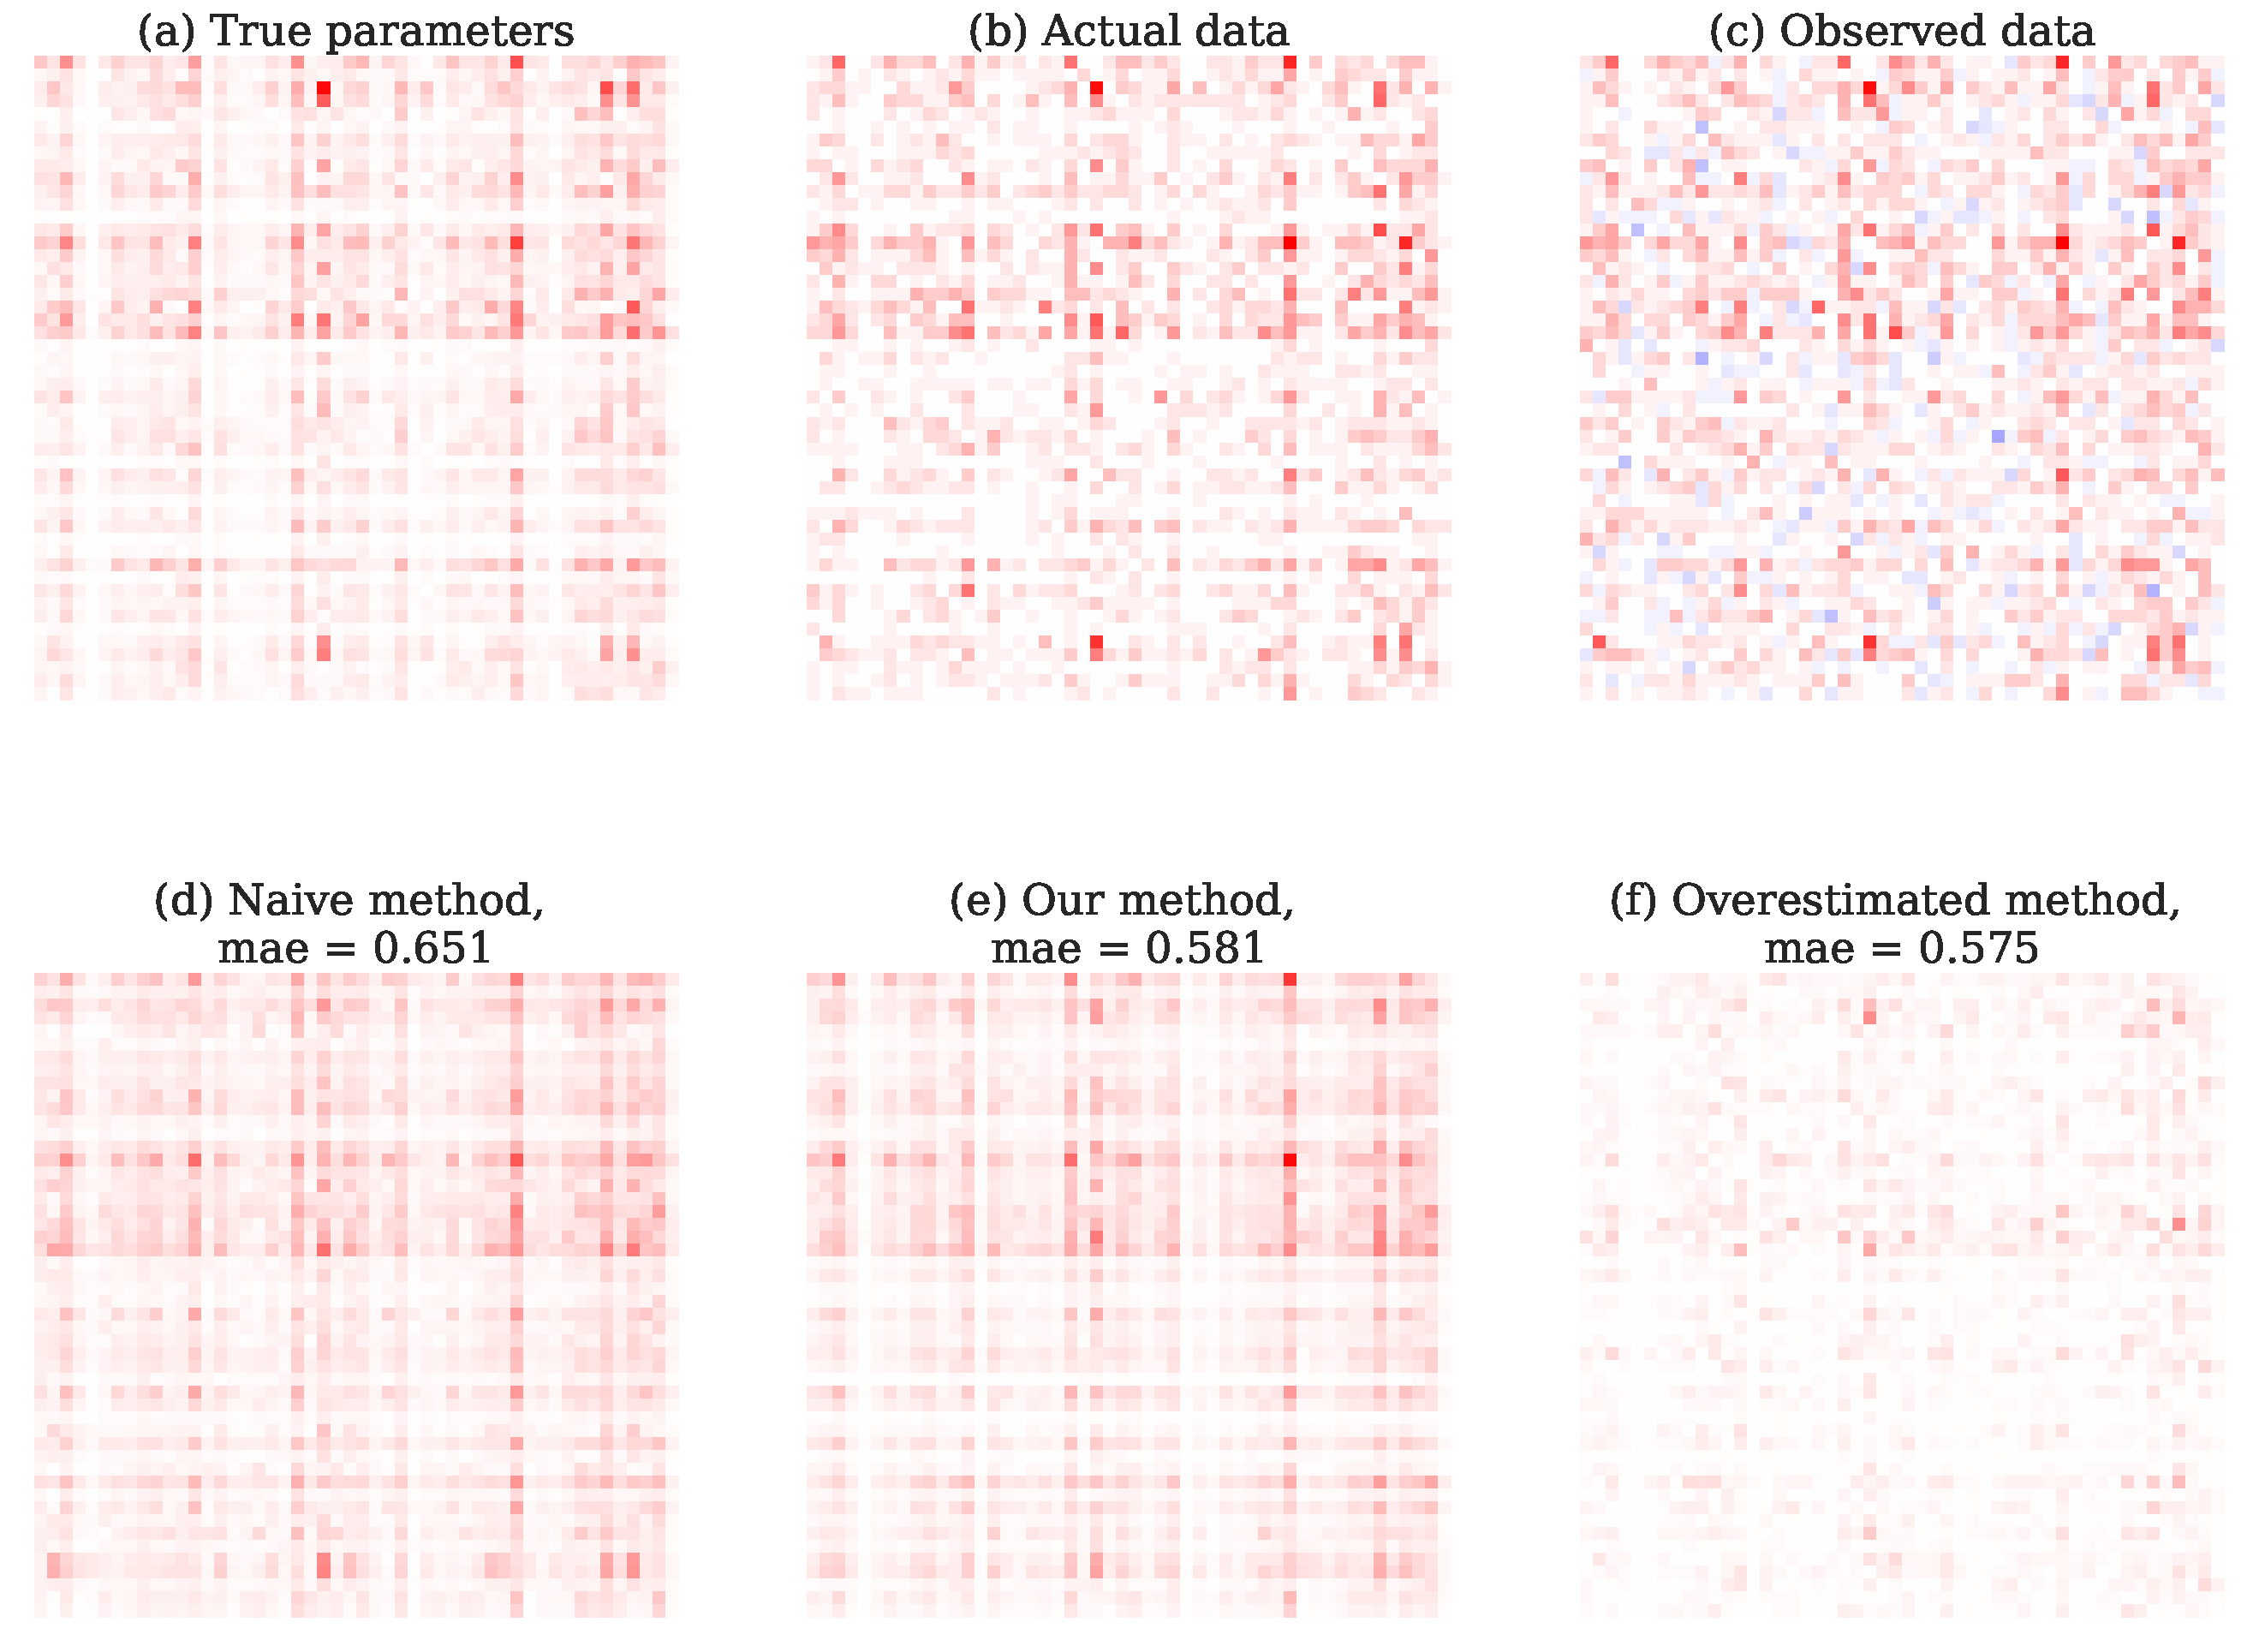
\includegraphics[width=0.95\textwidth]{figures/test_output.pdf}
    \caption{Demonstration of the results of the VI inference process for a
     50-word, 50-document synthetic dataset with 5 latent topics. The true
     data parameters (a) are recovered better by our inference procedure (e)
     than by naive variational inference (d), even though the noisy data (c)
     is much denser than the true data (b). Though inconsistent, in some random
     trials where we incorrectly informed the model that $\epsilon / N = 0.9$,
     our estimates of the prior, while lower-magnitude, would be closer to the
     true model.}
    \label{fig:test_output}
\end{figure*}
  %\section{Related Work} % DP, local privacy % Private topic models % Previous
  % work on VI for Poisson factorization
  
  % \section{Generative Processes} In a noiseless model, we assume we have a
  % tensor of true observed count data $\Yten$ with $M$ modes, each with a
  % dimension $d_1, \dots, d_M$. For standard Poisson tensor factorization, we
  % assume this data to be drawn from an entry-wise Poisson prior $\hat{\Yten}$
  % with a CP (Canonical Polyadic) decomposition into $M$ matrices $\theta^{(1)}
  % \dots \theta^{(M)}$ with a low-rank internal dimension $K$: 
  
  % \begin{equation} \Yten \sim \Pois{\Yten; \hat{\Yten}}, \text{ where }
  %     \hat{\Yten} = \sum_{k=1}^{K} \factori{1}_{:,k} \otimes \dots \otimes
  %     \factori{M}_{:,k}. \label{eq:bptf_full} \end{equation}
  
  % This is effectively the sum of $K$ rank-1 tensors of the same dimensions as
  % $\pmb{Y}$, where the $k$th rank-1 tensor in the sum is described as the
  % Kronecker product of the $k$th column vector of each factor matrix
  % $\factori{i}$. Note that the dimension of the $i$th mode factor matrix
  % $\factori{i}$ is $d_i \times k$. In Bayesian Poisson Tensor Factorization,
  % we also assume a Gamma prior over each of the latent factor matrices with
  % shape parameter $\alpha$ and rate $\alpha \beta$.\footnote{This
  % characterization ensures that the expectation of the Gamma distribution can
  % be expressed as a function of only $\beta$.}
  
  % Our algorithm applies \emph{limited-precision local privacy} to our data,
  % guaranteeing that for some maximum distance between private items $n$, it
  % will be statistically indistinguishable up to a factor $\epsilon$ of privacy
  % as to whether or not a given element is present in the original data. The
  % privacy algorithm we use takes in a tensor of privacy parameters $\pmb{E}$,
  % where each entry $\epsilon_{\subs}$ specifies the amount of privacy budget
  % required for entry $\ys$ in the true data. We can also generate a tensor
  % $\pmb{N}$ defining each $n_{\subs}$ as the maximum distance over which to
  % preserve privacy between $\ys$ and its neighbors.
  
  % To make our data private, we add two-sided geometric (2SG) noise
  % \cite{ghosh_universally_2012}. We use $\epsilon_{\subs}$ and $n_{\subs}$
  % values to compute our 2SG noise parameter $\alpha_{\subs}$: \begin{equation}
  % \alpha_{\subs} = n_{\subs} \ln{\frac{1}{\epsilon_{\subs}}}. \end{equation}
  % We can recharacterize 2SG noise as the difference between two Poisson
  % distributions, which offers one alternate way to write out our generative
  % process: for each entry $\ys$ in our unnoised data, we sample priors for the
  % each of the two Poisson noise variables $\lamP$ and $\lamM$ from an
  % exponential distribution of parameter $\frac{\alpha}{1 - \alpha}$. Then, we
  % sample $\gP$ from a Poisson of parameter $\lamP$, and $\gM$ likewise from
  % $\lamM$. The noise added is $\gP - \gM$.
  
  % Our final reported noisy data $\tilde{\Yten}$ is the tensor where geometric
  % noise has been added to each entry of the original tensor. These data should
  % be sparse (though less than before) and integer-valued, but they may not be
  % non-negative.
  
  % The model above ties together the two models through the $\Yten$ data: the
  % expectation of the true data from the privacy model inference can be used
  % directly in BPTF in place of the true data. Another way to tie the models
  % together, however, is through the inferred Poisson parameters $\hat{\Yten}$.
  % We can write a different generative procedure that generates $\gPM$ based on
  % the observation of the noisy data $\ytPM$ and the corresponding Poisson
  % prior $\ysh$. First, we use the Skellam distribution to sample $\ytPM$ using
  % the priors $\lamPM$ and $\Yten$ directly, with the same generative process
  % as before for these parameters. Then, we can sample the minimum $m$ of $\gM$
  % and $\ys + \gP$ from a Bessel distribution, observing that the difference
  % between these two is $\ytPM$.
  
  % The joint posterior of the above method is:
  
  % \begin{align} \begin{split} P(-) =\ &   % P distribution \Exp{\lamP;
  %     \frac{\alpha}{1 - \alpha}} \Exp{\lamM; \frac{\alpha}{1 - \alpha}}
  %     \Skel{\ytPM; \ysh + \lamP, \lamM}\\
  %         &\Bess{\omega_{\subs}; |\ytPM|, 2 \sqrt{(\ysh + \lamP) \lamM}} \\
  %         &\Multi{(\wsu{y}{1}, \dots, \wsu{y}{K}, \gP); \ytP,
  %         \left(\frac{\wsu{\hat{y}}{1}}{\ytP}, \dots,
  %         \frac{\wsu{\hat{y}}{K}}{\ytP}, \frac{\lamP}{\ytP} \right)} \\
  %         &\Delt{\ytP = \omega_{\subs}}^{\Delt{\ytPM \leq 0}} \Delt{\gM =
  %         \omega_{\subs}}^{\Delt{\ytPM > 0}} \Delt{\ytPM = \ytP - \gM}.
  %         \end{split} \end{align}
  
  % \section{Variational Procedure} In order to infer a variational inference
  % procedure for inferring a private Poisson factorization model, we wish to
  % ensure that all of the relevant distributions for our updates can be
  % expressed as exponential family. The Poisson, gamma, and exponential
  % distributions are all well-known exponential family distributions; however,
  % the Bessel distribution is not. However, we prove that the Bessel
  % distribution $m \!\sim\!\Bess(\nu, a)$ can be treated as an exponential
  % family function with a fixed $\nu$. This suits the scenario of our inference
  % procedure, where $\nu$ is defined by the true data $\ytPM$, which is
  % observed at inference time.
  
  % \subsection{Privacy parameter updates} % Lambdas come from gamma variational
  % parameters delta and gamma % Many of our parameters are redundant, so we
  % just focus on inferring m, the true y_dvk, and lambdas % Lambda rate is
  % constant, so just need shape for lambda^{\pm} Unfortunately, the natural
  % $q$-distribution for $m$ causes problems for typical inference.
  % Specifically, it requires using $\Expect[\ytP]$ as the number of samples
  % from a binomial distribution, which could be a non-integer. Instead, we
  % replace the $q$-distribution with a delta spike centered on the \emph{mode}
  % of the Bessel distribution whose arguments are defined as before. While the
  % mode and mean of the Bessel are not equal, the mode is still within a small
  % constant range of the arithmetic expectation of $m$:
  
  % \begin{equation} \big| \Expect [\Bess{m; a, \nu}]  - \text{mode}(\Bess{m; a,
  %     \nu}) \big|  \leq 1. \end{equation}
  
  % The intuitive meaning of this is that the mode of the Bessel distribution is
  % guaranteed to be one of the two integers closest to the mean of the
  % distribution. (We omit the proof here for the sake of concision.) This makes
  % the mode a natural integer substitute to use for the real-valued expectation
  % of the Bessel distribution in settings where we need integral values. %
  % define Q using delta-spike using mode instead of mean, prove ok (Xanda) % To
  % handle m, we use a mode approximation (which we can prove is close % to the
  % mean) % True y_dvk fall out from this
  
  % \subsection{Poisson Factorization parameter updates} % These updates are
  % basically the same as before, just conditioned on the true y_dvk inferred
  % from the process above
  
  % \subsection{Computing the ELBO} % Copy from elsewhere (Aaron?)
  \section{Validation}
  \label{sec:validation}

  In order to test this result, we generated synthetic count data using a
  Poisson matrix factorization formulation analogous to the LDA topic model
  \citep{blei2003latent} with $D$ documents, $V$ unique terms in a document
  vocabulary, and $K$ latent topics. We first used a Gamma prior to generate two
  matrices of latent parameters, $\theta$ of dimension $D \times K$ and $\phi$
  of dimension $K \times V$. We then compute the product of these, $\theta \phi
  = \Yten$, as the Poisson prior of our data generation process. Finally, we add
  two-sided geometric noise scaled to $\epsilon / N = 1$, a ratio that applies
  when the privacy budget $\epsilon$ and the maximum allowed difference between
  documents $N$ are equal (e.g., a privacy budget of 2 to privatize 2-word
  spans). We then test our inference procedure to see how closely it estimates
  the true parameters of the original model. We find that our model successfully
  converges to within a reasonable estimate of the true model parameters given
  the data, as demonstrated in a small example in Figure \ref{fig:test_output}.
  
  
  Using a larger example of a synthetic 1000-by-1000 matrix of count
  observations, we test the performance of this algorithm as compared to the
  performance using inference with MCMC \citep{schein2018locally}. We observe
  that a single-threaded version of the code from the MCMC implementation, even
  with optimizations such as reducing the frequency of parameter resampling for
  the noise distributions, each iteration of inference takes approximately 0.8
  seconds. Using 4000 iterations of burnin and 1000 to collect samples with 32
  cores, we are able to take the combined inference time down to 6 minutes
  (using 200 minutes of observed CPU time), with a final mean average error
  (MAE) of 0.208. In contrast, our variational inference model takes
  approximately 2.8 seconds per iteration, and requires only 41-42 iterations to
  converge across ten trials, resulting in a combined 1 minute of inference (15
  minutes of observed CPU time) to reach an error of 0.395.  

  \section{Discussion}
  We present a new CAVI algorithm for inference of Bayesian Poisson
  factorization models under local privacy. Our method relies on two key
  theoretical insights about the Bessel distribution: first, that with fixed
  $\nu$, it belongs to the exponential family, and second, that its mode is an
  integer neighbor of its mean. Using these, we implement a tool with
  significant performance improvements over even an optimized version of the
  prior MCMC algorithm. On a synthetic test case of inferring a rank-50
  factorization of an 1000 by 1000 data observation matrix, we obtain a 12x
  speedup in model inference over convergence of the MCMC method. Though the
  standard version of our privacy-aware method produces error similar to the
  naive, non-private implementation of MCMC Bayesian Poisson factorization, we
  can produce improved results by overestimating the amount of private noise
  that was added, forcing additional sparsity into the model. Further, we can
  use this VI procedure as initialization for an MCMC model to improve
  performance.
  
  \bibliographystyle{plainnat}
  \bibliography{uai_2019}
  
  \appendix
  
  \section{The Bessel distribution as exponential family}
  \label{sec:expfambessel}
  
  \textbf{Theorem 1}
    \label{theorem:expfam}
    \textit{The Bessel distribution $m \!\sim\!\textrm{Bes}(\nu, a)$ for fixed
   $\nu$ is an exponential family with sufficient statistic $T_\nu(m) \teq 2m
   \tp \nu$, natural parameter $\eta_\nu(m) \teq \log\left(\frac{a}{2}\right)$,
   and base measure $h_\nu(m) \teq \frac{1}{m!\,\Gamma(m+\nu+1)}$.}
  \begin{proof}
  The Bessel distribution \citep{yuan2000bessel} is a two-parameter distribution
  over the non-negative integers:
  \begin{equation}
  f(n; a, \nu) = \frac{\left(\frac{a}{2}\right)^{2n+\nu}}{n!\, \Gamma(n{+}\nu{+}1) I_\nu(a)},
  \end{equation}
  where the normalizing constant $I_\nu(a)$ is a modified Bessel function of the
  first kind---i.e.,
  \begin{equation}
  I_\nu(a) = \sum_{n=0}^\infty
  \frac{\left(\frac{a}{2}\right)^{2n+\nu}}{n!\, \Gamma(n{+}\nu{+}1)}.
  \end{equation}

  For fixed and known $\nu$, we can rewrite the Bessel PMF as
  \begin{align}
    f(n; a, \nu) =&
    \frac{1}{n!\,\Gamma(n{+}\nu{+}1)} \notag\\
    &\exp\left((2n{+}\nu)\,\log\left(\frac{a}{2}\right)
    -\log I_\nu(a)\right).
    \end{align}

  We can then define the following functions:
  \begin{align}
  h_\nu(n) &= \frac{1}{n!\,\Gamma(n{+}\nu{+}1)} \\
  T_\nu(n) &= 2n+\nu\\
  \eta_\nu(a) &= \log\left(\frac{a}{2}\right) \\
  A_\nu(a) &= \log I_\nu(a).
  \end{align}

  Finally, we can rewrite the Bessel PMF in the exponential-family form:
  \begin{equation}
  f(n; a, \nu) = h_\nu(n) \exp{\left(\eta_\nu(a) \cdot T_\nu(n) -
  A_\nu(a)\right)}.
  \end{equation}
  \end{proof}
  
  \section{The mode and mean of the Bessel distribution}
  \label{sec:besselmode}
  
  \textbf{Proposition 3}
    \label{theorem:besselmode}
    \textit{The mode of a Bessel distribution for parameters $a, \nu$ can be a constant-bounded approximation of the mean:}
  
  \[
      \big| \mathbbm{E}_{\Bess{m; \nu, a})}[m]  - \textup{mode} \left(\Bess{m; a, \nu} \right) \big|  \leq 1.  
  \]
  
  The intuitive meaning of this is that the mode of the Bessel distribution is
  guaranteed to be one of the two integers closest to the mean of the
  distribution. Given one of these two integers will always be the best integer
  approximation of this number, we can also say that there cannot exist an
  integer approximation of the mean of the Bessel that is strictly between the
  mode and the mean of the Bessel distribution.
  
  \begin{proof}
  
  A Bessel distribution takes two arguments, which we refer to as its \besv,
  $\nu$ and \besa, $a$. The distribution is defined as:
  
  \begin{align}
      p(x = n~&|~x \sim \Bess{\nu, a})\notag \\
      &= \frac{1}{I_{\nu}(a)n!\Gamma(n + \nu + 1)} \left( \frac{a}{2} \right)^{2n + \nu},   
  \end{align}
  where $I_{\nu}(a)$ is a modified Bessel function of the first kind. The
  arithmetic mean of the distribution is
  \[
      \mathbbm{E}_{\Bess{m; \nu, a})}[m] = \frac{a}{2} R_{\nu}(a),
  \]
  with $R_{\nu}(a)$ referring to the ratio of two Bessel functions:
  \[
      \frac{I_{\nu + 1}(a)}{I_{\nu}(a)}.
  \]
  
  The Bessel distribution has one or two neighboring integer modes. The mode can
  be computed directly from the parameters of the distribution without Bessel
  functions:
  \[
      \textup{mode}(\Bess{\nu, a}) = \bigg \lfloor \frac{\sqrt{a^2 + \nu^2} - \nu}{2} \bigg \rfloor.
  \]
  Unlike the mean, which can take arbitrary non-negative real values, the mode
  is guaranteed by the floor function to be a non-negative integer.
  
  We use the following bound on the mean of a Bessel ratio from
  \citet{devroye2002simulating}:
  
  \begin{equation}
      \frac{a}{\nu + 1 + \sqrt{a^2 + (\nu + 1)^2}} \leq R_{\nu}(a)
      \leq \frac{a}{\nu + \sqrt{a^2 + \nu^2}}.
  \end{equation}
  
  We multiply through by $\frac{a}{2}$ to bound the mean of the Bessel
  distribution:
  
  \begin{equation}
      \frac{a^2}{2(\nu + 1 + \sqrt{a^2 + (\nu + 1)^2})} \leq \mathbbm{E}_{\Bess{m; \nu, a})}[m]
      \leq \frac{a^2}{2(\nu + \sqrt{a^2 + \nu^2})}.
  \end{equation}
  
  We can rewrite these bounds using a difference-of-squares:
  
  \begin{align*}
      \frac{a^2}{2(\nu + \sqrt{a^2 + \nu^2})} &= 
      \frac{a^2(\sqrt{a^2 + \nu^2} - \nu)}{2(\nu + \sqrt{a^2 + \nu^2})(\sqrt{a^2 + \nu^2} - \nu)} \\
      &= \frac{a^2(\sqrt{a^2 + \nu^2} - \nu)}{2a^2 + \nu^2 - \nu^2} \\
      &= \frac{\sqrt{a^2 + \nu^2} - \nu}{2}.
  \end{align*}
  
  This upper bound coincides with the unrounded formulation of the mode. Because
  the mode is the floor of this quantity, we know it is less than or equal to
  this upper bound with a difference of less than 1.
  
  We can convert the lower bound in the same way:
  \begin{equation*}
      \frac{a^2}{2((\nu + 1) + \sqrt{a^2 + (\nu^2 + 1)})} =  \frac{\sqrt{a^2 + (\nu + 1)^2} - (\nu + 1)}{2}.
  \end{equation*}
  
  We are interested in bounding the difference between the upper and lower
  bounds:
  \begin{equation}
      \frac{\sqrt{a^2 + \nu^2} - \nu}{2} - \frac{\sqrt{a^2 + (\nu + 1)^2} - (\nu + 1)}{2} = 
      \frac{\sqrt{a^2 + \nu^2} + 1 - \sqrt{a^2 + (\nu + 1)^2}}{2}.
  \end{equation}
  
  Knowing that $\nu$ is positive, we can state that $\sqrt{a^2 + \nu^2} <
  \sqrt{a^2 + (\nu + 1)^2}$, or $\sqrt{a^2 + (\nu + 1)^2} - \sqrt{a^2 + \nu^2} >
  0$. Based on the upper slice of the triangle in the figure below, the triangle
  inequality also gives us another bound, that $\sqrt{a^2 + \nu^2} + 1 >
  \sqrt{a^2 + (\nu + 1)^2}$, or $1 > \sqrt{a^2 + (\nu + 1)^2} - \sqrt{a^2 +
  \nu^2}$.
  
  \begin{center}
  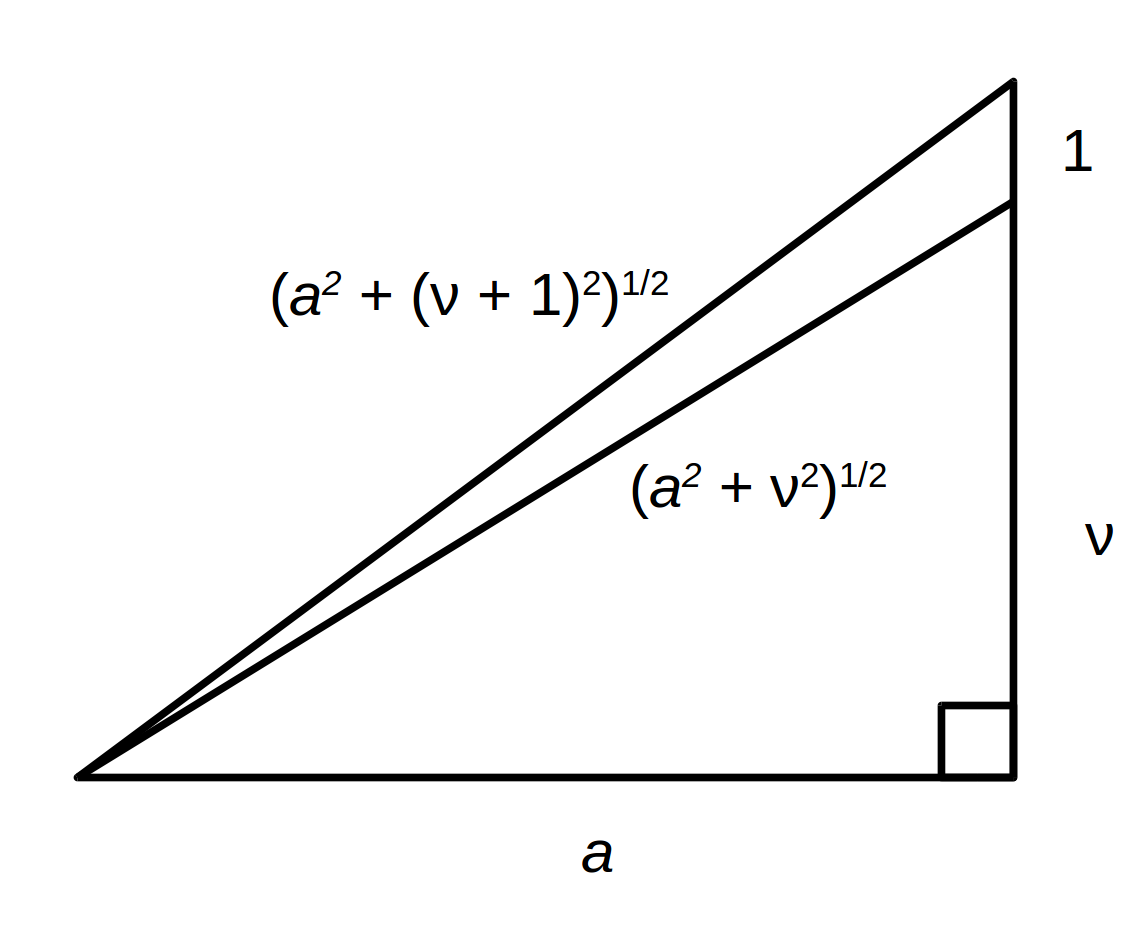
\includegraphics[width=0.3\textwidth]{figures/triangle-bessel-model}
  \end{center}
  Together, these imply that 
  \[
      0 \leq \sqrt{a^2 + \nu^2} + 1 - \sqrt{a^2 + (\nu + 1)^2} \leq 1.
  \]
  
  Substituting this in to our computation of the distance between the upper and
  lower bounds of the mean, we find that
  \begin{equation}
  \frac{\sqrt{a^2 + \nu^2} + 1 - \sqrt{a^2 + (\nu + 1)^2}}{2} < \frac{1}{2},
  \end{equation}
  
  or that the inferred upper and lower bounds for the mean of the Bessel
  distribution produce an interval no larger than $\frac{1}{2}$. The upper bound
  of this $\frac{1}{2}$ interval is the same as the upper bound of the length-1
  open interval of the mode of the Bessel. In the most extreme case when the
  mode is at the bottom end of its range and the mean is at the top, we have
  \[
      \mathbbm{E}_{\Bess{m; \nu, a})}[m] - \textup{mode}(\Bess{\nu, a}) < 1.
  \]
  In the opposite case, we have 
  \[
      \textup{mode}(\Bess{\nu, a}) - \mathbbm{E}_{\Bess{m; \nu, a})}[m] \leq \frac{1}{2} < 1.
  \]
  \end{proof}
  
  
  
  

\end{document}
